\documentclass{standalone}
\usepackage{tikz}
\usetikzlibrary{arrows.meta, decorations.markings, intersections, positioning}

\begin{document}
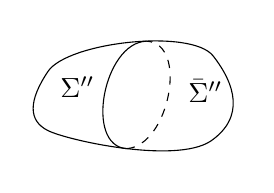
\begin{tikzpicture}[scale=.25]

\begin{scope}[scale=.05, xshift=-170cm, yshift=-111cm]
    \draw   (170,111) .. controls (190,101) and (299,77) .. (335,100) .. controls (371,124.5) and (360,158.5) .. (338,186.75) .. controls (316,215) and (190,201) .. (170,171) .. controls (150,141) and (150,121) .. (170,111) -- cycle ;
\end{scope}

\draw  (4,-.92) to [in=182, out=176] +(1,5.46);
\draw [dashed] (4,-.92) to [in=-2, out=4] +(1,5.46);

\node at (1.5,2.2) {$\Sigma''$};
\node at (8, 2) {$\bar{\Sigma}''$};

\end{tikzpicture}
\end{document}